\documentclass[runningheads]{llncs}

\let\proof\relax
\let\endproof\relax
\usepackage{amsmath,amsthm,amssymb}
\usepackage{tikz, tikz-cd}

\newcommand{\A}{\mathcal{A}}
\newcommand{\G}{\mathcal{G}}
\renewcommand{\P}{\mathfrak{A}}
\newcommand{\C}{\mathfrak{C}(\Am,\e)}
\newcommand{\Z}{\mathbb{Z}}
\newcommand{\Q}{\mathbb{Q}}
\newcommand{\2}{\textbf{2}}
\newcommand{\Am}{\textbf{A}}
\newcommand{\del}{\partial}
\newcommand{\vv}{\bar{v}}
\newcommand{\e}{\bar{e}}
\newcommand{\T}{\mathcal{T}}

\newtheorem{thm}{Theorem}

\title{Extensions of Abelian Automata Groups}
\author{Chris Grossack\orcidID{0000-0001-7520-9747}}

\institute%
{%
  Carnegie Mellon University, Pittsburgh, USA\\
  \email{cgrossac@andrew.cmu.edu}
}

\begin{document}
\maketitle

\begin{abstract}
  A longstanding problem in understanding abelian automata groups
  comes from a seemingly unnecessary parameter in the classification
  given by Nekrashevich and Sidki. In this paper, we show that
  this parameter corresponds to the presence of certain fractional group
  elements. Further, we show the existence of a computable universal object 
  which removes the need for this parameter entirely.

  \keywords{Abelian Automata \and Transducer \and Module Theory}
\end{abstract}


\section{Background}
Finite State Automata are combinatorial objects which encode relations 
between words over some alphabet. Automata provide deep connections between
combinatorics, algebra, and logic, and are essential tools in contemporary 
computer science. One such link is in the decidability of truth in a structure
whose relations are all computable by automata. One can combine these automata 
into more complicated automata representing logical sentences in such a way 
that a sentence is true if and only if a simple reachability condition holds
\cite{Brny07:automatic_structures}. This gives a simple proof that the theory 
of $\mathbb{N}$ with $+$ and $<$, for example, is decidable.

While the most common automata one encounters are DFAs
and Turing Machines, providing a characterization of the complexity of 
certain languages, automata can encode functions, and therefore groups,
as well. These groups are surprisingly complicated, and indeed a 
classification of all groups generated by three state automata over the 
alphabet $\2 = \{0,1\}$ is an extremely difficult problem, though much
impressive progress has been made \cite{Bondarenko09:three_state}. This
complexity can be extremely useful, as automaton groups have become a rich
source of examples and counterexamples
\cite{Nekrashevych05:self_similar_groups%
     ,Sidki00:one_rooted_trees%
     ,GrigorchukNS00:automata_groups%
     }. 
Automaton groups provide examples of
finitely generated infinite torsion groups, with application to 
Burnside's Problem \cite{Gupta83:burnside}, and automata groups have
provided the only examples of groups of intermediate growth, providing 
counterexamples to Milnor's Conjecture regarding the existence of such groups
\cite{Grigorchuk11:Milnor}. In fact, one of the simplest conceivable automata 
(shown below) already generates the lamplighter group $\Z/2\Z \wr \Z$
\cite{GrigorchukZuk01:lamplighter}.

\begin{center}
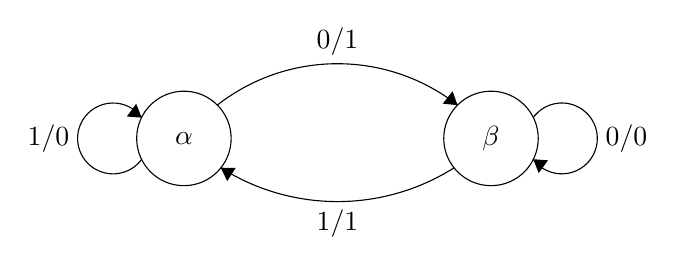
\begin{tikzpicture}[scale=0.2]
\tikzstyle{every node}+=[inner sep=0pt]
\draw [black] (15.8,-29.2) circle (3);
\draw (15.8,-29.2) node {$\alpha$};
\draw [black] (35.3,-29.2) circle (3);
\draw (35.3,-29.2) node {$\beta$};
\draw [black] (13.12,-30.523) arc (-36:-324:2.25);
\draw (8.55,-29.2) node [left] {$1/0$};
\fill [black] (13.12,-27.88) -- (12.77,-27) -- (12.18,-27.81);
\draw [black] (17.918,-27.085) arc (128.02449:51.97551:12.39);
\fill [black] (33.18,-27.09) -- (32.86,-26.2) -- (32.24,-26.99);
\draw (25.55,-23.96) node [above] {$0/1$};
\draw [black] (37.98,-27.877) arc (144:-144:2.25);
\draw (42.55,-29.2) node [right] {$0/0$};
\fill [black] (37.98,-30.52) -- (38.33,-31.4) -- (38.92,-30.59);
\draw [black] (32.957,-31.065) arc (-57.68311:-122.31689:13.856);
\fill [black] (18.14,-31.06) -- (18.55,-31.91) -- (19.09,-31.07);
\draw (25.55,-33.71) node [below] {$1/1$};
\end{tikzpicture}
\end{center}

Because of the complexity of general automaton groups, in this paper we
restrict our attention to the abelian case, over the alphabet $\2$. 
For our purposes, then, a \textbf{Mealey Automaton} is a tuple $\A = (S, \tau)$
where $S$ is the \textbf{State Set}, and $\tau : S \times \2 \to S \times \2$ 
is the \textbf{transition function}. 
Given a state $s \in S$, we can treat it as a length preserving function 
$\underline{s} : \2^* \to \2^*$ as follows:
\begin{align*}
  \underline{s}(\varepsilon) &= \varepsilon\\
  \underline{s}(ax)       &= a' \underline{s'}(x) 
  ~~~(\text{where } (s', a') = \tau(s,a))
\end{align*}
Here juxtaposition is concatenation, and the empty word $\varepsilon$ is
the identity in $\2^*$. Clearly we can treat 
$\underline{s}$ as a function on $\2^\omega$, the set of infinite words, 
instead. In this case, automata provide a computable way of encoding 
complicated continuous functions from cantor space to itself, with ties to
descriptive set theory \cite{skrzypczak15:descriptive}.
If all of these functions are invertible, we let $\G(\A)$ denote
the group generated by these functions, with extra structure given by 
residuation (we write our groups additively, and denote the identity 
element by $I$). 

The \textbf{0-residual} (resp. \textbf{1-residual}) of a 
function $f \in \G(\A)$ is the unique function 
$\del_0 f$ such that for all $w$, $f(0w) = f(0) \del_0 f(w)$ 
(resp. $f(1w) = f(1) \del_1 f(w)$). 
For a state $s \in S$, it is clear that 
$\del_a \underline{s} = \underline{s'}$, where $(s',a') = \tau(s,a)$.
Since the generators are closed under residuation, so too is the group.
We will call a function \textbf{Odd} if it flips its first bit, and 
\textbf{Even} otherwise, and we call an automaton \textbf{Abelian} or \textbf{Trivial}
exactly when its group is. We represent $\tau$ graphically by labeling an
edge from $s_1$ to $s_2$ by $a/b$ exactly when $\tau(s_1,a) = (s_2,b)$.

So in the above automaton, $\underline{\alpha}$ is odd, $\underline{\beta}$ 
is even, $\del_0 \underline{\alpha} = \underline{\beta}$, 
and $\del_1 \underline{\alpha} = \underline{\alpha}$.
Further,
$\underline{\alpha}(011) = 1\underline{\beta}(11) = 11\underline{\alpha}(1) = 110$.
For a more in depth description of Mealy Automata and their properties, 
see \cite{Sakarovitch09:automata_theory,Holcombe}.

Of great importance to abelian automata theory is the result of 
Nekrashevich and Sidki that every such group is either torsion free abelian or 
boolean \cite{NekrashevychSidki04:automorphisms}. Because of this classification, 
much of the interesting structure of these groups comes from the residuation
functions. To that end, for the duration of this paper, 
homomorphisms and isomorphisms are all restricted to those 
which preserve the residuation structure in addition to the group structure.
It is a theorem by Sutner \cite{Sutner18:abelian_automata} 
that $\G(\A)$ is abelian iff for even states $\del_1 f - \del_0 f = I$ 
and for odd states $\del_1 f - \del_0 f = \gamma$, where $\gamma$ is 
independent of $f$. Moreover, the case $\gamma = I$ corresponds 
precisely to the case where $\G(\A)$ is boolean.
We now restrict ourselves further to the case where $\G(\A)$ is 
free abelian, that is to say $\G(\A) \cong \Z^m$ for some $m$,
and $\gamma \not = I$.%
\footnote%
{%
  For historical reasons we use $\Z^m$ instead of $\Z^n$ because 
  traditionally $n$ is reserved for the size of the state set of 
  an automaton.
}

It was shown by Nekrashevich and Sidki \cite{NekrashevychSidki04:automorphisms} 
that $\Z^m$ itself can be considered the state set of an automaton.
The odd (resp. even) states are exactly the vectors with odd (resp. even) 
first component. To define the transition function, we require a 
$\frac{1}{2}-integral$ matrix $\Am$ of $\Q$-irreducible character. 
This automaton group is generated by a \emph{finite} automaton exactly if 
$\Am$ is a contraction (that is, all of its complex eigenvalues 
should have norm $<1$). By a $\frac{1}{2}-integral$ matrix, we mean a matrix 
of the form

\[
\begin{pmatrix}
  \frac{a_{11}}{2} & a_{12} & \dots  & a_{1n}\\
  \vdots           & \vdots & \ddots & \vdots\\
  \frac{a_{n1}}{2} & a_{n2} & \dots  & a_{nn}\\
\end{pmatrix}
\]
where each $a_{ij} \in \Z$. These matrices all have characteristic polynomial\\
$\chi = x^n + \frac{1}{2}g(x)$, where $g \in \Z[x]$ and has constant term 
$\pm 1$.\\ 
Since $\Am : 2\Z \oplus \Z^{m-1} \to \Z^m$,
residuation acts as multiplication by $\Am$ for even vectors,
but for odd vectors we need to first make them even. To that end, let $\e$
be odd, and define residuation as follows:

If $\vv$ is even:
\[ \del_0 \vv = \del_1 \vv = \Am \vv \]

If $\vv$ is odd:
\[ \del_0 \vv = \Am (\vv - \e) \]
\[ \del_1 \vv = \Am (\vv + \e) \]
Following Sutner \cite{Sutner18:abelian_automata}, we call this 
\textbf{The Complete Automaton} $\C$. 

Each $\G(\A)$ can also be viewed as an automaton, by taking $\G(\A)$ 
as states, and defining $\tau(f,i) = \del_i f$. $\A$ is a natural subautomaton
of $\G(\A)$ by identifying $s \in \A$ with $\underline{s} \in \G(\A)$.
Nekrashevich and Sidki's theorem gives us a purely linear algebraic method
of discussing these automaton groups, since a restatement of their theorem 
says that every torsion free abelian automaton group $\G(\A)$ is isomorphic 
to $\C$ for some $\Am$ and $\e$, and therefore every abelian automaton $\A$
is a subautomaton of some $\C$. $\Am$ is easily seen to be unique up to 
GL($\Q$) similarity, and so we call it the \textbf{Associated Matrix} of $\A$.
However there are infinitely many valid choices for $\e$, and classifying 
these is the goal this paper. We say a function $f \in \G(\A)$ is 
\textbf{Located at} $\vv \in \C$ iff the isomorphism between $\G(\A)$ and 
$\C$ sends $f$ to $\vv$. Further, given any state $\vv \in \C$, closing 
$\{ \vv \}$ under residuation will result in a finite automaton $\A_{\vv}$ 
since $\Am$ is a contraction. So we say an automaton $\A$ is \textbf{Located At} 
$\vv \in \C$ iff the isomorphism sends $\A$ to $\A_{\vv} \subseteq \C$. 
Note that the location of a function or an automaton, and indeed whether a 
location exists or not, will depend on the choice of $\e$. For a more detailed
discussion of these linear algebraic methods and their origins, see
\cite{Nekrashevych05:self_similar_groups,NekrashevychSidki04:automorphisms}

\subsection{Principal Automata}
To each abelian automaton we can associate a matrix as above, however each
matrix can be associated to infinitely many automata.
It was shown by Okano \cite{Okano15:thesis} that there is a 
distinguished automaton, now called the \textbf{Principal Automaton} $\P$, 
associated to each matrix. $\P(\Am)$ is defined to be 
$\P = \A_{\e_1} \cup \A_{-\e_1} \subseteq \mathfrak{C}(\Am, \e_1)$,
though there is a longstanding conjecture that in most cases this is
the same machine as $\A_{\e_1} \subseteq \mathfrak{C}(\Am, \e_1)$.
We will write $\P$ when the matrix is clear from context. 

We shall soon see that the same element of $\P$ is located at $\e$ in 
$\C$ for all $\e$, and so we call this group element $\delta \in \G(\P)$. 
Notice that for all $\e$, $\del_0 \delta = \Am(\e - \e) = \bar{0} = I$, and so
$\del_1 \delta = \gamma$, since for any odd vector 
$\del_1 \vv - \del_0 \vv = \gamma$. Thus, $\gamma$ depends on only the 
matrix $\Am$, rather than on individual automata.

$\P$ is clearly minimal in terms of state complexity, as its states are
distinct group elements of $\mathfrak{C}(\Am, \e_1)$ and therefore 
definitionally have different behavior. However, $\P$ is also minimal in the
subgroup relation for nontrivial automata sharing its matrix. 
While there are proofs of this claim which rely heavily on the
ambient linear algebraic structure \cite{Okano15:thesis}, 
we present here a difference construction which uses only the given 
automaton $\A$ to construct $\P$. Thus every $s \in \P$ is already in
$\G(\A)$, and the subgroup relation follows.

\begin{thm}
  For each nontrivial $\A$ with associated matrix $\Am$,\\
  $\G(\P(\Am)) \leq \G(\A)$.
\end{thm}

\begin{proof}
  Let $\A$ be an abelian automaton with at least one odd state.
  Note that if $\A$ has no odd states, its group is trivial, so we may
  safely ignore it.

  Put $\gamma = \del_1 f - \del_0 f$ for $f \in \A$ odd, and construct
  a new automaton by closing $\gamma$ under residuation.
  Note that this can be done using only information contained in $\A$,
  since it is easy to check that:
  \[
    \del_0(f + g) = \begin{cases} \del_0 f + \del_1 g & \text{both odd}\\
                                  \del_0 f + \del_0 g & \text{otherwise}
                    \end{cases}
  \]
  \[
    \del_1(f + g) = \begin{cases} \del_1 f + \del_0 g & \text{both odd}\\
                                  \del_1 f + \del_1 g & \text{otherwise}
                    \end{cases}
  \]
  \[
    \del_0 (-f) = - \del_1 f
  \]
  \[
    \del_1 (-f) = - \del_0 f
  \]

  Thus using the characterization by Sutner \cite{Sutner18:abelian_automata}, 
  that a state is odd iff it has distinct residuals, we can close $\gamma$ 
  under residuation using only information in $\A$.
  Since $\gamma \in \G(\A)$ and $\G(\A)$ is residuation closed, 
  this entire closure is a subset of $\G(\A)$. 

  Another theorem by Sutner \cite{Sutner18:abelian_automata} says that 
  adding a state which residuates into an existing automaton does not 
  change the group. To that end, the above closure generates the same group
  as the above closure with an additional state $\delta$ residuating into 
  $\gamma$ and a self loop $I$. This new machine is exactly 
  $\A_{\e_1} \subseteq \mathfrak{C}(\Am,\e_1)$. Any state in $\A_{\-e_1}$ is
  the negation of a state in $\A_{e_1}$, and so 
  $\P(\Am) = \A_{\e_1} \cup \A_{-\e_1} \subseteq \G(\A)$. 
  Then $\G(\P(\Am)) \leq \G(\A)$, as desired.
\end{proof}



\subsection{An Example}
Consider the following machine, $\A^3_2$:

\begin{center}
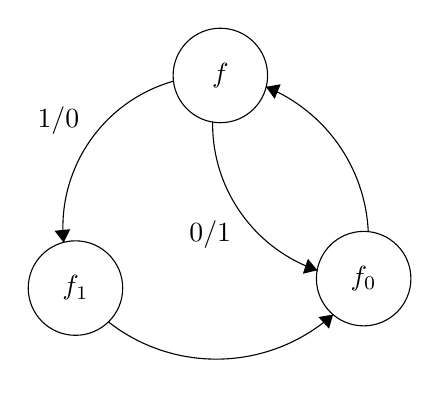
\begin{tikzpicture}[scale=0.2]
\tikzstyle{every node}+=[inner sep=0pt]
\draw [black] (26.6,-12.1) circle (3);
\draw (26.6,-12.1) node {$f$};
\draw [black] (17.4,-25.6) circle (3);
\draw (17.4,-25.6) node {$f_1$};
\draw [black] (35.7,-25) circle (3);
\draw (35.7,-25) node {$f_0$};
\draw [black] (16.648,-22.708) arc (-174.31762:-254.2298:9.658);
\fill [black] (16.65,-22.71) -- (17.07,-21.86) -- (16.07,-21.96);
\draw (17.67,-14.97) node [left] {$1/0$};
\draw [black] (33.761,-27.277) arc (-48.14861:-128.09563:11.117);
\fill [black] (33.76,-27.28) -- (32.83,-27.44) -- (33.5,-28.18);
\draw [black] (29.501,-12.822) arc (67.8011:2.5992:10.451);
\fill [black] (29.5,-12.82) -- (30.05,-13.59) -- (30.43,-12.66);
\draw [black] (32.758,-24.474) arc (-108.88288:-180.71682:9.832);
\fill [black] (32.76,-24.47) -- (32.16,-23.74) -- (31.84,-24.69);
\draw (27.31,-22.21) node [left] {$0/1$};
\end{tikzpicture}
\end{center}

Here the unlabeled transitions both copy the input bit, however these
have been omitted for cleanliness.

Then by letting $\gamma = \del_1 f - \del_0 f = f_1 - f_0$, and closing
under residuation using the above algorithm, we construct the following 
machine ($\gamma$ is shown at the bottom left): 

\begin{center}
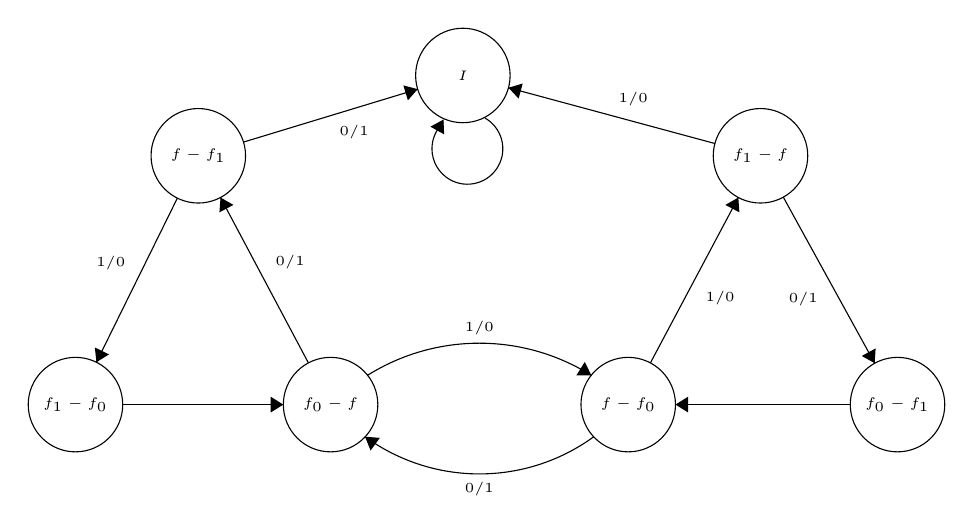
\begin{tikzpicture}[scale=0.2]
\tikzstyle{every node}+=[inner sep=0pt]
\draw [black] (36.4,-15.9) circle (3);
\draw (36.4,-15.9) node {\tiny $I$};
\draw [black] (37.8,-18.6) arc (60.34019:-227.65981:2.25);
\fill [black] (35.17,-18.7) -- (34.34,-19.15) -- (35.21,-19.64);
\draw [black] (55.3,-21) circle (3);
\draw (55.3,-21) node {\tiny $f_1-f$};
\draw [black] (64,-36.8) circle (3);
\draw (64,-36.8) node {\tiny $f_0-f_1$};
\draw [black] (46.9,-36.8) circle (3);
\draw (46.9,-36.8) node {\tiny $f-f_0$};
\draw [black] (28,-36.8) circle (3);
\draw (28,-36.8) node {\tiny $f_0-f$};
\draw [black] (11.8,-36.8) circle (3);
\draw (11.8,-36.8) node {\tiny $f_1-f_0$};
\draw [black] (19.6,-21) circle (3);
\draw (19.6,-21) node {\tiny $f-f_1$};
\draw [black] (22.47,-20.13) -- (33.53,-16.77);
\fill [black] (33.53,-16.77) -- (32.62,-16.53) -- (32.91,-17.48);
\draw (29.5,-19.03) node [below] {\tiny $0/1$};
\draw [black] (18.27,-23.69) -- (13.13,-34.11);
\fill [black] (13.13,-34.11) -- (13.93,-33.61) -- (13.03,-33.17);
\draw (15,-27.81) node [left] {\tiny $1/0$};
\draw [black] (14.8,-36.8) -- (25,-36.8);
\fill [black] (25,-36.8) -- (24.2,-36.3) -- (24.2,-37.3);
\draw [black] (26.59,-34.15) -- (21.01,-23.65);
\fill [black] (21.01,-23.65) -- (20.94,-24.59) -- (21.83,-24.12);
\draw (24.48,-27.74) node [right] {\tiny $0/1$};
\draw [black] (30.345,-34.939) arc (122.03013:57.96987:13.397);
\fill [black] (44.56,-34.94) -- (44.14,-34.09) -- (43.61,-34.94);
\draw (37.45,-32.4) node [above] {\tiny $1/0$};
\draw [black] (52.4,-20.22) -- (39.3,-16.68);
\fill [black] (39.3,-16.68) -- (39.94,-17.37) -- (40.2,-16.41);
\draw (47.22,-17.84) node [above] {\tiny $1/0$};
\draw [black] (56.75,-23.63) -- (62.55,-34.17);
\fill [black] (62.55,-34.17) -- (62.61,-33.23) -- (61.73,-33.71);
\draw (58.98,-30.09) node [left] {\tiny $0/1$};
\draw [black] (61,-36.8) -- (49.9,-36.8);
\fill [black] (49.9,-36.8) -- (50.7,-37.3) -- (50.7,-36.3);
\draw [black] (48.31,-34.15) -- (53.89,-23.65);
\fill [black] (53.89,-23.65) -- (53.07,-24.12) -- (53.96,-24.59);
\draw (51.78,-30.06) node [right] {\tiny $1/0$};
\draw [black] (44.711,-38.841) arc (-53.966:-126.034:12.343);
\fill [black] (30.19,-38.84) -- (30.54,-39.72) -- (31.13,-38.91);
\draw (37.45,-41.7) node [below] {\tiny $0/1$};
\end{tikzpicture}
\end{center}

It is easy to check that this is the principal machine for
$\Am = \begin{pmatrix} -1 & 1 \\ -\frac{1}{2} & 0 \end{pmatrix}$,
and further that $\A^3_2$ as above is located at 
$\e_1 \in \mathfrak{C}\left ( \Am, \begin{pmatrix} 3 \\ 2 \end{pmatrix} \right )$

When running the algorithm in this case, we do not need to separately add
$\pm \delta$ or the inverse machine. Here $\delta = f - f_1$, and the machine
is already closed under negation. The Strongly Connected Component Conjecture 
predicts that this will be the case whenever $\Am$ has characteristic 
polynomial other than $x^m - \frac{1}{2}$, which corresponds to the so called 
sausage automata. Unfortunately, however, this conjecture is yet unproven,
and so in the above proof we had to explicitly add in these extra states.

\section{Group Extensions}
Going forward, $\G = \Z^m$ will denote $\G(\P)$ for some principal machine $\P$.

$\G$ clearly admits representation as a $\Z[x]$ module where 
$x \cdot \vv = \Am^{-1}\vv$, extended linearly. Further, since $\Am$ has 
irreducible character so does $\Am^{-1}$. Thus this module is cyclic, 
and is generated by $\e_1 = \delta$. 
(Note that since $\Am$ sends $2\Z \oplus \Z^{m-1}$ to $\Z^m$, and therefore
has multiples of $\frac{1}{2}$ in general, $\Am^{-1}$ sends $\Z^m$ to 
$2\Z \oplus \Z^{m-1}$, and so has only integer entries).

Now for $p \in \Z[x]$ with odd constant term, we write
$p \cdot \G$ in place of\\ $\G(\mathfrak{C}(\Am,p \cdot \e_1))$.
That is to say, $p \cdot \G$ has as its states $\Z^m$ and as its 
odd residuations
$\del_0 \vv = \Am (\vv - p \cdot \e_1)$, and 
$\del_1 \vv = \Am (\vv + p \cdot \e_1)$.
Since this module is cyclic, every $\vv$ arises as 
$p_{\vv} \cdot \e_1$ where 
$p_{\vv} = \vv_0 + \vv_1 x + \ldots + \vv_{m-1} x^{m-1}$.
We will only discuss polynomials $p$ with an odd constant term, as 
this ensures $p \cdot \e_1$, our residuation vector, is odd.

We call $p \cdot \G$ the \textbf{Group Extension} of $\G$ by $p$.
To justify this nomenclature, we first notice 
$\G \hookrightarrow p \cdot \G$ for all $p$ by the
homomorphism $\vv \mapsto p \cdot \vv$. 
Further, we recognize that if $p$ is not a unit in 
$\text{End}_{\G} \cong \Z^m / \chi^*$, this homomorphism is \emph{not} 
surjective. That is to say $\G$ is a proper subgroup of $p \cdot \G$.
Here, $\text{End}_{\G}$ is the ring of all group endomorphisms, not 
necessarily preserving the residuation structure, and $\chi^*$ is the
characteristic polynomial of $\Am^{-1}$. 
This observation is true in more generality, as shown below.

\begin{thm}
  If $rp = q$ in $\Z[x]$, then $p \cdot \G \hookrightarrow q \cdot \G$, 
  with a canonical injection $\varphi_r : \vv \mapsto r \cdot \vv$. 
  In particular, if $r$ is a unit, then $p \cdot \G \cong q \cdot \G$.
\end{thm}

\begin{proof}
  Let $rp = q$, $f \in p \cdot \G$ located at $\vv$. 
  Consider $f' \in q \cdot \G$ located at $r \cdot \vv$.

  First note $f$ and $f'$ have the same parity, since 
  $r$ has odd constant term, and so $\vv$ and $r \cdot \vv$
  have the same parity. Now, consider the residuals of $f$ and $f'$. 
  
  If $f$ is even, then 
  \[ \del_0 f' = \Am (r \cdot \vv) = r \cdot \Am \vv = r \cdot \del_0 f \]

  If $f$ is odd, then
  \[ \del_0 f' = \Am (r \cdot \vv - q \cdot \e_1) 
               = r \cdot \Am (\vv - p \cdot \e_1)
               = r \cdot \del_0 f \]

  A similar argument shows $\del_1 f' = r \cdot \del_1 f$

  If $r$ is a unit, then $r^{-1}$ also has odd constant term 
  (since $r * r^{-1} = 1$ has odd constant term) and so $\varphi_r$
  is an isomorphism with inverse $\varphi_{r^{-1}}$.
\end{proof}

\section{Fractional Elements}
As the previous proof shows, $p \cdot \vv \in p \cdot \G$, 
computes exactly the same function as $\vv \in \G$.
However, most vectors cannot be written as $p \cdot \vv$. 
What do they do as functions?
We call such vectors (and their corresponding functions)
\textbf{Fractional}, due to the following observation and theorem:

Consider $\e_1 \in 3 \cdot \G$. By the above theorem, $3\e_1 = \delta$,
and so we should expect $\e_1$ to behave like ``$\frac{1}{3}\delta$'', 
and in fact it does.

In general, $\vv \in p \cdot \G$ behaves like $p^{-1} \cdot \vv \in \G$,
(where $p^{-1}$ comes from $\Q[x]$ and so $p^{-1} \cdot \vv \in \Q^m$)
and so Group Extensions give us access to fractions of functions from 
our base group $\G$.

We will consider $p^{-1} \cdot \Z^m = \{ p^{-1} \cdot \vv~|~\vv \in \Z^m \}$
as a subgroup of $\Q^m$. Residuation in this setting is given by
$\del_0 \vv = \Am (\vv - \e_1)$ and $\del_1 \vv = \Am (\vv + \e_1)$.
Here, instead of scaling \emph{up} our residuation vector, 
we scale \emph{down} all of our other vectors. Then we have access to 
certain elements of $\Q^m$, which are exactly the factional elements
as noted before. Now $\delta$ is always located at $\e_1$.

Morally, however, this is just a different way of looking at the group 
extension construction. We justify this with the following theorem:

\begin{thm}
  For $p \in \Z[x]$ with odd constant term, 
  $p^{-1} \cdot \Z^m \cong p \cdot \G$.
\end{thm}

\begin{proof}
  Consider $\varphi : p^{-1} \cdot \Z^m \to p \cdot \G$ by
  $\varphi(p^{-1} \cdot \vv) = \vv$.\\
  $\varphi$ is clearly bijective, and is a homomorphism since:
  \begin{align*}
       \varphi(p^{-1} \cdot \vv_1 + p^{-1} \cdot \vv_2) 
    &= \varphi(p^{-1} \cdot (\vv_1 + \vv_2))\\
    &= \vv_1 + \vv_2\\
    &= \varphi(p^{-1} \cdot \vv_1) + \varphi(p^{-1} \cdot \vv_2) 
  \end{align*}

  Further, if $\vv$ is even, then:

  \begin{align*}
       \varphi(\del_0 (p^{-1} \cdot \vv))
    &= \varphi(\Am (p^{-1} \cdot \vv))\\
    &= \varphi(p^{-1} \cdot \Am \vv)\\
    &= \Am \vv\\
    &= \del_0 (\varphi(p^{-1} \cdot \vv))
  \end{align*}

  If $\vv$ is odd, then: 

  \begin{align*}
       \varphi(\del_0 (p^{-1} \cdot \vv))
    &= \varphi(\Am (p^{-1} \cdot \vv - \e_1))\\
    &= \varphi(p^{-1} \cdot \Am (\vv - p \cdot \e_1))\\
    &= \Am (\vv - p \cdot \e_1)\\
    &= \del_0 (\varphi(p^{-1} \cdot \vv))
  \end{align*}

  The proof for $\del_1$ is similar.
\end{proof}

Thus we can view functions in $p \cdot \G$ as fractions of functions in $\G$.
It is a natural question to ask which fractions are attainable in this way.

Clearly, for any $f \in \G$, we can attain $\frac{1}{k} f$ for any odd $k$.
Simply take $\vv \in k \cdot \G$ for $f$ located at $\vv$.
However, fractions with even denominator are, in general, unattainable.
$2 \frac{1}{2}\delta = \delta$ should be an odd function,
but no function, when doubled, is odd.

\section{Characterizing Automata}
Since each automaton $\A$ is a subautomaton of some $\C$,
equivalently some $p \cdot \G$, there should be a minimal $\e$ 
(up to multiplication by units) which still has $\A$ as a subautomaton. 

Notice that if we locate $\A$ at $\e_1 \in p \cdot \G$, 
then there can be no smaller polynomial $q$ (in the division ordering)
which also places $\A$ at an integral position. The following theorem 
shows this is always possible.

\begin{thm}
  Every nontrivial abelian automaton $\A$ can be 
  located at $\e_1$ in $p \cdot \G$ for some $p$.
\end{thm}

\begin{proof}
  It is a theorem by Sutner \cite{Sutner18:abelian_automata} that every 
  finite state abelian automaton residuates into a strongly connected component, 
  and further that this component generates the same group as the entire 
  machine. So we may, with no loss of generality, assume our machine is 
  strongly connected (that is, every state except possibly $I$ has a path to
  every other state).

  Let $f$ be an odd state in $\A$. Then at least one of $\del_0 f$ and 
  $\del_1 f$ is not equal to $f$. So there is some nontrivial cycle
  from $f$ to itself, which we can represent by a matrix equation 
  relating $\vv_f$, and $\e$. (Here $\vv_f$ is where $f$ will be located, 
  and $\e$ will be the residuation vector). 
  We can then rearrange this equation to obtain 
  $p_1(\Am)\vv_f = p_2(\Am)\e$.

  $p_1, p_2 \in \Z[x]$, and $\Am$ has irreducible character over $\Z$.
  It is well known that the eigenvalues of $p(\Am)$ are precisely $p(\lambda)$
  where $\lambda$ is an eigenvalue of $\Am$, so $\Am$'s invertibility implies
  the invertibility of both $p_1(\Am)$ and $p_2(\Am)$. Thus

  \[ \e = p_2(\Am)^{-1}p_1(\Am)\vv_f \]

  Choosing $\vv_f = \e_1$ gives a value for the residuation vector $\e$,
  and (since $\G$ is cyclic as a $\Z[x]$ module) a value $\e$ induces a 
  polynomial $p_{\e}$ such that $p_{\e} \cdot \e_1 = \e$. 
  Then, by construction, $\A$ is a subautomaton of $p_e \cdot \G$, and is 
  anchored with $f$ at $\e_1$. As desired.
\end{proof}

For any automaton $\A$, we can now completely characterize in
which $\C$ it can be located, and at what vectors.
Simply locate $\A$ at $\e_1 \in p \cdot \G$, and then to locate it at
any odd vector $\vv$, scale both sides by $p_{\vv}$ to see $\A$ located at
$\vv \in p_{\vv} p \cdot \G$. 
In the above proof, the choice of $\vv_f = \e_1$ was arbitrary, and we can
directly locate $\A$ at a different odd vector $\vv'$ by setting 
$\vv_f = \vv'$. This will give the same result as locating it at $\e_1$ and 
then multiplying by $p_{\vv'}$, again, by cyclicity.
The same observation shows that, given some polynomial $q$ 
(equivalently some vector $q \cdot \e_1$) $\A$ is located somewhere in 
$q \cdot \G = \mathfrak{C}(\Am,q \cdot \e_1)$ if and only if $p \mid q$. 
Further, it will be located at exactly $p^{-1}q \cdot e_1$.

\subsection{An Example}
Recall the abelian automaton $\A^3_2$ from earlier in the paper:

\begin{center}
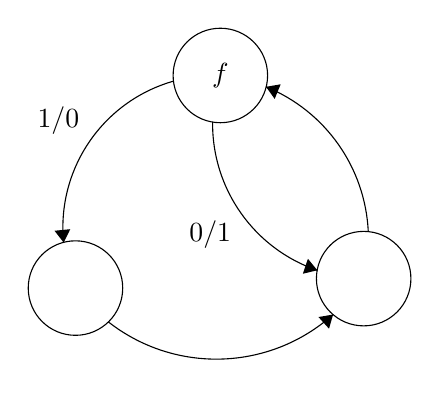
\begin{tikzpicture}[scale=0.2]
\tikzstyle{every node}+=[inner sep=0pt]
\draw [black] (26.6,-12.1) circle (3);
\draw (26.6,-12.1) node {$f$};
\draw [black] (17.4,-25.6) circle (3);
\draw [black] (35.7,-25) circle (3);
\draw [black] (16.648,-22.708) arc (-174.31762:-254.2298:9.658);
\fill [black] (16.65,-22.71) -- (17.07,-21.86) -- (16.07,-21.96);
\draw (17.67,-14.97) node [left] {$1/0$};
\draw [black] (33.761,-27.277) arc (-48.14861:-128.09563:11.117);
\fill [black] (33.76,-27.28) -- (32.83,-27.44) -- (33.5,-28.18);
\draw [black] (29.501,-12.822) arc (67.8011:2.5992:10.451);
\fill [black] (29.5,-12.82) -- (30.05,-13.59) -- (30.43,-12.66);
\draw [black] (32.758,-24.474) arc (-108.88288:-180.71682:9.832);
\fill [black] (32.76,-24.47) -- (32.16,-23.74) -- (31.84,-24.69);
\draw (27.31,-22.21) node [left] {$0/1$};
\end{tikzpicture}
\end{center}

Say we want to find $\vv$ and $\e$ such that $\A^3_2$ is located at 
$\vv \in \C$.

Using the algorithm described by Becker \cite{Becker18:thesis} gives 
$\Am = \begin{pmatrix} -1 & 1 \\ -\frac{1}{2} & 0 \end{pmatrix}$.

Then notice $\del_0 \del_0 f = f$.
So $\Am^2 (\vv_f - \e) = \vv_f$, and
$\Am^2 \vv_f - \vv_f = \Am^2 \e$. Thus

\[ \e = \Am^{-2} (\Am^2 - I) \vv_f \]

Choosing $\vv_f = \e_1$ gives $\e = \begin{pmatrix} 3 \\ 2 \end{pmatrix}$.

Then $f = \begin{pmatrix} 1 \\ 0 \end{pmatrix} \in (3+2x) \cdot \G$

\subsection{Limiting Object}
Since each $p \cdot \G$ can be viewed as $p^{-1} \cdot \Z^m \subseteq \Q^m$
with residuation vector $\e_1$,
it is reasonable to consider the subgroup of $\Q^m$
\[ 
  \widetilde{\G} = \bigcup_p p^{-1} \cdot \Z^m 
\]
(Recall we only include polynomials with odd constant term in this union)

Notice that this group is universal, in the sense that it contains as
subgroups each $p \cdot \G$. Further, it concretely shows the relationships
between the various automata. In this setting, we see exactly why automata 
show up in multiple group extensions, and why the division ordering of 
polynomials is the characterizing factor. $p \cdot \G$ is an approximation
of $\widetilde{\G}$, where we scale up by a factor of $p$ and take only
the integral vectors (residuation is necessarily scaled up to match). 
In this structure, then, there is no unnecessary duplication of the location
of automata, and there is no extra parameter $\e$.

\section{Conclusion}
We have shown that the residuation vector $\e$ corresponds to how fine an
approximation of $\widetilde{\G}$ one wants. This is because each $\C$ 
corresponds to $p_{\e} \cdot \G$, with progressively larger $\e$ 
corresponding to progressively more complicated fractional elements, which
approximate $\widetilde{\G}$. Thus, the parameter really provides a way of
interacting with these elements living in $\Q^m$ as though they were in $\Z^m$,
and so by computing in $\widetilde{\G}$ (or a suitably large approximation) 
directly, we can remove the need for this parameter.

Further, the existence of the universal object $\widetilde{\G}$ 
sheds new light on the connection between affine tiles
\cite{LagariasWang96:tiles,LagariasWang97:integral_tiles}
and abelian automata noted by Sutner
\cite{Sutner18:abelian_automata}. 
Indeed it is easy to see that in 
$\widetilde{\G}$ every strongly connected component 
(and thus every subautomaton of interest) has each vector in the attractor 
of the iterated function system given by the residuation functions 
$\{ \vv \mapsto \Am \vv, \vv \mapsto \Am (\vv \pm \e_1) \}$.
Thus, in particular, the size of the principal machine is bounded by the
number of integral points in this attractor. Even in $\Z^2$, however, there
are examples where this bound is not tight.

The relation between automata and polynomials discussed in this paper 
also provides a new take on a proof technique for the longstanding
Strongly Connected Component Conjecture. This conjecture 
asserts that principal machines $\P$ have only one strongly connected component 
(plus the self looping identity state) whenever their matrix has a 
characteristic polynomial that is \emph{not} of the form $x^n + \frac{1}{2}$.
The new way of looking at residuation vectors allows us to rewrite the 
residual functions as $\del_i \vv = \Am (\vv - (-1)^i \delta)$ for $\vv$ odd.
It is easy to see, then, that the following polynomials correspond to paths
ending in $\delta$, since they undo residuation:

\begin{align*}
  P_\epsilon(x)   &= 1\\
  P_{w0}(x)       &= xP_w(x) + 0\\
  P_{w1}(x)       &= xP_w(x) + 1\\
  P_{w\bar{1}}(x) &= xP_w(x) - 1
\end{align*}

Sutner made a similar observation, and described Path Polynomials 
\cite{Sutner18:abelian_automata} which
allow us to reason about the existence of directed paths between states 
in an automaton by purely algebraic means. However, these polynomials are
clunky and not always defined, since they correspond to paths
\emph{starting} at $\delta$, and so $P'_{w0} \cdot \delta$ is only well 
defined if $P'_w \cdot \delta$ is even (and $P'_{w1}$ and $P'_{w\bar{1}}$ 
are only well defined if $P_w \cdot \delta$ is odd). Since the polynomials 
defined above move \emph{backwards} along transitions instead of forwards, 
they are always well defined.

The existence of a path polynomial $p$ which is congruent to $-1$ mod $\chi^*$
then shows the existence of a path from $-\delta$ to $\delta$.
Then to prove the SCC conjecture, it suffices to prove that whenever $\Am$ 
does not have characteristic $x^n + \frac{1}{2}$ there is a polynomial 
$p \in \{-1,0,1\}[x]$ which is congruent to $-1$ mod $\chi^*$. 
Efforts are underway to use this method to actually prove the conjecture.

\section*{Acknowledgements}
This paper would not exist without the advice of my advisor Klaus Sutner.
There aren't enough thanks for the hours of conversation I enjoyed.

\newpage

\bibliographystyle{splncs04}
\bibliography{bib}

\end{document}
